\documentclass[../index.tex]{subfiles}
\begin{document}
\section{Что такое динамическая форма?}
\emergencystretch 3em
Динамическая форма состоит из набора динамических полей, представленных в древовидной структуре.
Поля представляют собой стандартные элементы UI: поля ввода текста, чекбоксы, раскрывающиеся списки, кнопки и т. д.
Они взаимодействуют между собой, с пользователем и внешними системами,
что в конечном счете позволяет автоматизировать любой бизнес процесс.

На низком уровне динамическая форма описана следуя синтаксису XML.
Рассмотрим пример простейшего шаблона динамической формы:
\begin{verbatim}
    <form>
        <text id="helloworld"
              label="Простое текстовое поле"
              mandatory="false"
              sbcommand=""
              sbcopyinfo="false"
              sbfield=""
              sbmask=""
              sbmodify="true"
              sbstyle=""
              sbtask=""
              sbtitle=""
              sbtype=""
              setGroupId=""
              style="text"
              type="2"
              visible="true" width=""></text>
    </form>
\end{verbatim}

В пользовательском интерфейсе портала «Лицо ДРУГа», динамическая форма будет выглядеть так:

\begin{figure}[h]
	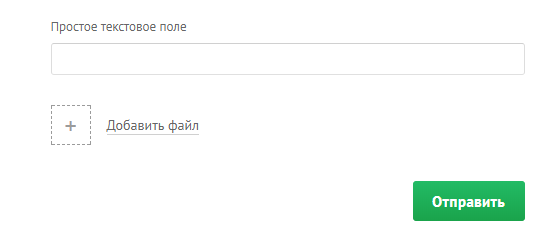
\includegraphics[width=1.0\textwidth]{simpleDynamicForm}
	\centering
\end{figure}

\textbf{Примечание}

Заметьте, что на изображении присутствуют элементы интерфейса «Добавить файл» и «Отправить».
Они не описаны в динамической форме и являются стандартными для всех шаблонов.
Но все же поля динамической формы имеют возможность управлять состоянием этих «статических» элементов
при помощи функций динамического языка.

\section{Конструктор динамических форм}
Во главе концепций динамических форм ставилась скорость и легкость их разработки/сопровождения.
Но написание даже самой простой динамической формы в XML – непростая задача.
Необходимо определить множество свойств, полей, событий и отслеживать взаимосвязи между ними.

Для упрощения процесса создания динамической формы был разработан удобный графический конструктор
динамических форм на платформе HP Service Manager:

\begin{figure}[h]
	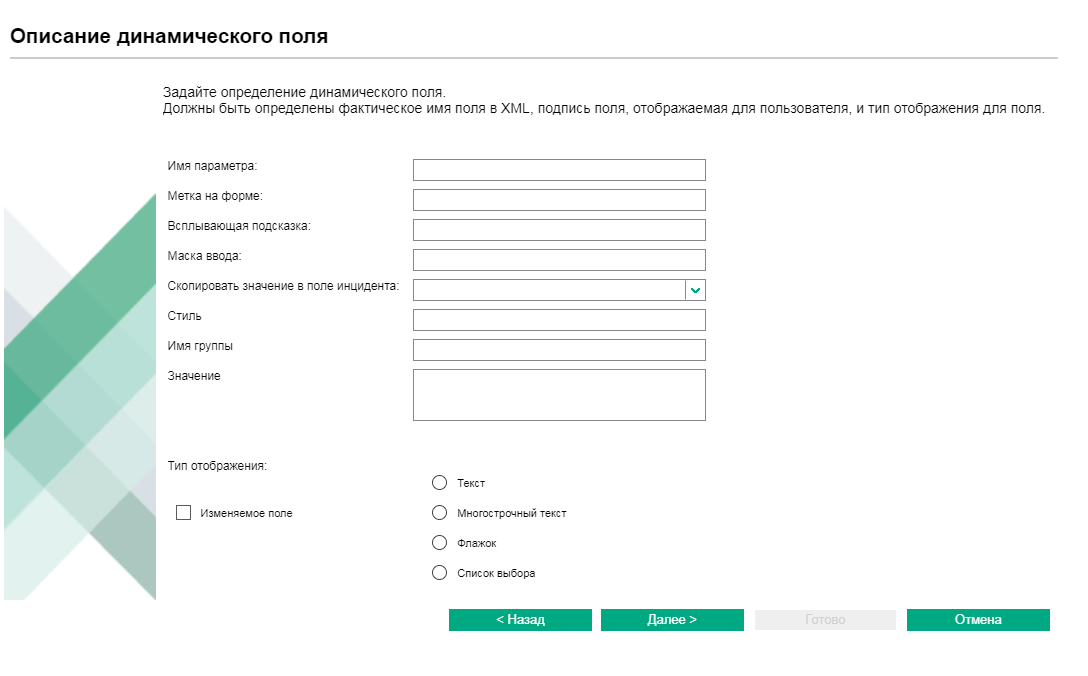
\includegraphics[width=1.0\textwidth]{dynamicFormConstructor}
	\centering
\end{figure}

Описание конструктора динамических форм, выходит за рамки данной книги.
Его интерфейс интуитивно понятен, поэтому не вызовет трудностей в освоении,
даже для людей без опыта в разработке UI.

\section{Режимы открытия динамических форм}
Динамические формы поддерживают несколько режимов работы:

\begin{enumerate}
	\item \verb|MODE_CREATE_INTERACTION| -- режим создания нового обращения из шаблона
	\item \verb|MODE_OPEN_INTERACTION| -- режим чтения обращения
    \item \verb|MODE_OPEN_INCIDENT| -- режим работы с инцидентом
	\item \verb|MODE_COPY_TEMPLATE| -- режим копирования обращения
\end{enumerate}

\subsection{MODE\_CREATE\_INTERACTION}
В режиме создания обращения возможность редактирования полей устанавливается 
флагом \verb|sbmodify| в элементах шаблона: если он равен \verb|true| -- то динамическое поле доступно для редактирования, если такую возможность подразумевает типа данного поля.
При открытии шаблона выполняются динамические команды, указанные в свойствах  \verb|sbcommand| динамических
полей последовательно, в порядке их объявления в шаблоне. Кнопка <<Создать обращение>> отображается по умолчанию
	
\subsection{MODE\_OPEN\_INTERACTION}
В режиме чтения обращения все поля по умолчанию закрыты для редактирования, флаг \verb|sbmodify| игнорируется.
Для <<Разблокирования>> некоторых полей существует механизм \verb|unreadEditableFields| -- данный атрибут обращения содержит массив идентификаторов динамических полей, которые будут доступны для редактирования в данном режиме. Команды \verb|sbcommand| выполняются только в разблокированных полях, вместо них отрабатывают команды из атрибутов \verb|sbonload| динамических полей. Кнопка <<Сохранить обращение>> отображается только в том случае, если массив \verb|unreadEditableFields| непустой.

\section{Наследование состояния\\динамической формы}
Ранее упоминалось, что динамическая форма после исполнения и преобразований пользователя,
сохраняет свое состояние в БД. Из этого состояния может быть создана «производная» динамическая форма,
которая будет наследовать некоторые свойства исходной. Эта возможность бывает очень полезной,
когда мы хотим освободить пользователя от необходимости повторно заполнять одинаковые динамические поля.

Под наследованием состояния динамической формы, понимается последовательный перенос свойств динамических полей
из исходной формы в производную. Перенос производится для динамических полей, совпадающих по свойству \verb|id|.

Наследуются следующие свойства: \verb|value|, \verb|visible|, \verb|enabled|, \verb|sbmodify|.

\textbf{Примечание}

Некоторые типы динамических элементов, содержат значения в виде набора дочерних элементов,
например: чек-боксы, радио-боксы, выпадающие списки. Эти дочерние элементы имеют свои
свойства: видимость, доступность для редактирования и значение.
Свойства дочерних элементов тоже должны быть унаследованы, и передаются в
атрибутах: \verb|valueSelected|, \verb|valueEnabled|, \verb|valueVisible|.

Существует три способа наследовать состояние:

\begin{enumerate}
	\item копирование динамической формы (кнопка «Копировать»);
	\item создание связанного обращения;
    \item передача свойств динамической формы, через ссылку в аргументах URL.
\end{enumerate}

\subsection{Кнопка «Копировать»}
Бизнес услуги могут быть востребованы пользователем несколько раз за короткий промежуток времени.
Пользователь, заполняет форму (обращения) получения услуги один раз, а далее создает копию этого обращения
и лишь незначительно меняет его поля. Для этого, в режиме просмотра обращения (по некоторым услугам),
доступна кнопка «Копировать».

TODOFIXME

\section{Общее описания динамического поля}
	Каждое динамическое поле представляет собой набор стандартных и дополнительных параметров отвечающих за визуальное отображение и функциональное поведение элемента.
	Определение элемента задается при формировании шаблонов в HPSM, разнообразие типов достигается комбинацией значений параметров \textbf{sbtype}, \textbf{type}, \textbf{logicalType}, \textbf{objectType}, \textbf{logicalType}
	В качестве примера приведем простое текстовое поле:
\begin{verbatim}
	{
		"objectType": "text",
		"logicalType": "text",
		"id": "editmarriagenumauto",
		"label": "Свидетельство о браке",
		"mandatory": false,
		"sbcommand": "",
		"sbmask": "",
		"sbmodify": true,
		"sbtask": "",
		"sbtitle": "например \"VI-МЮ-777777\"",
		"sbtype": "",
		"sbstyle": "width:33%",
		"style": "text",
		"visible": false,
		"width": "",
		"sbobject": null,
		"sbdbfield": null,
		"sbaction": null,
		"sbmode": null,
		"sbonload": null,
		"sbcopyinfo": false,
		"childs": null,
		"groupid": "",
		"text": null,
		"options": null,
		"type": "2",
		"multiline": null,
		"button": null,
		"matchTable": null,
		"matchField": null,
		"query": null,
		"hpcGroupByFields": null,
		"sbfield": ""
	}
\end{verbatim}
	и элемент типа select:
\begin{verbatim}
	{
		"objectType": "select",
		"logicalType": "combo",
		"id": "purpose",
		"label": "Цель поездки",
		"mandatory": true,
		"sbcommand": "setvalue([something],[purpose])",
		"sbmask": "",
		"sbmodify": true,
		"sbtask": "setvalue([something],[purpose])",
		"sbtitle": "",
		"sbtype": "",
		"sbstyle": "",
		"style": "combo",
		"visible": true,
		"width": "",
		"sbobject": null,
		"sbdbfield": "purpose",
		"sbaction": null,
		"sbmode": null,
		"sbonload": "setvalue([something],[purpose])",
		"sbcopyinfo": false,
		"children": null,
		"groupid": "",
		"text": "Встречи с клиентами",
		"options": [
			{
			"text": "Выезды на аварии",
			"label": "id02",
			"id": "id02"
			},
			{
			"text": "Встречи с клиентами",
			"label": "Встречи с клиентами что-т там",
			"id": "id03"
			},
			{
			"text": "Выезды в государственные органы",
			"label": "Выезды в государственные органы",
			"id": "id04"
			}
		],
		"type": "2",
		"multiline": null,
		"button": null,
		"matchTable": null,
		"matchField": null,
		"query": null,
		"hpcGroupByFields": null,
		"sbfield": ""
	}
\end{verbatim}
\subsection{Параметры динамического поля}
\begin{enumerate}
	\item \verb|objectType| - параметр отвечающий за определение типа поля
	\item \verb|logicalType| - параметр отвечающий за определение типа поля
	\item \verb|sbtype| - параметр отвечающий за определение типа поля
	\item \verb|type| - параметр отвечающий за определение типа поля
	\item \verb|style| - параметр отвечающий за определение типа поля
	\item \verb|id| - уникальный идентификатор поля используется в командах динамического языка для поиска элемента
	\item \verb|text| - значение поля по умолчанию
	\item \verb|label| - заголовок поля, отображаемое значение для информации и обозначения поля
	\item \verb|sbtitle| - подсказка для поля, содержит дополнительную информацию о поле, выводиться в виде вопроса
	\item \verb|groupid| - параметр сортировки и формирования для плоских и legacy групп
	\item \verb|sbcommand| - содержит команды динамического языка выполняемые при инициализации \verb|MODE_CREATE_INTERACTION|
	\item \verb|sbtask| - содержит команды динамического языка выполняемые при изменении поля через пользовательский ввода
	\item \verb|sbonload| - содержит команды динамического языка выполняемые при инициализации \verb|MODE_OPEN_INTERACTION| или \verb|MODE_OPEN_INCIDENT|
	\item \verb|mandatory| - флаг отвечающий за обязательность поля
	\item \verb|sbmask| - маска поля ввода(используется для текстовых полей и дат)
	\item \verb|sbmodify| - флаг определяющий можно ли изменять поле
	\item \verb|sbstyle| - параметр отвечающий за визуальные стили элемента вызывает команду setStyle над элементом
	\item \verb|visible| - флаг определяющий видимость поля в пользовательском интерфейсе
	\item \verb|width| - значение в \% ширины элемента относительно блока
	\item \verb|sbobject| - HP SM property, не изменяется в рамках обработки
	\item \verb|sbdbfield| - HP SM property, не изменяется в рамках обработки
	\item \verb|sbaction| - HP SM property, может быть изменено командой setAction
	\item \verb|sbmode| - HP SM property, может быть изменено командой setMode
	\item \verb|sbcopyinfo| - флаг отвечающий за копирование значения динамического поля в физическое поле information 
	\item \verb|children| - дочерние элементы используется в элементе типа group
	\item \verb|options| - варианты значений для поля для полей с выбором значений
	\item \verb|multiline| - флаг отвечающий за возможность многострочного ввода для текстовых полей
	\item \verb|button| - HP SM property, не изменяется в рамках обработки
	\item \verb|matchTable| - HP SM property, не изменяется в рамках обработки
	\item \verb|matchField| - HP SM property, не изменяется в рамках обработки
	\item \verb|query| - HP SM property, не изменяется в рамках обработки
	\item \verb|hpcGroupByFields| - HP SM property, не изменяется в рамках обработки
	\item \verb|sbfield| - HP SM property, не изменяется в рамках обработки
\end{enumerate}

\subsection{Управление состоянием}

\section{Текстовые поля}
	Текстовые поля могут быть четырех разных визуальных типов + все поля для которых не определены правила тоже преобразуются в обычное текстовое поле
	\begin{enumerate}
		\item Обычное текстовое поле
		\item Неизменяемое текстовое поле(Label) - текстовое поле с флагом \textbf{modify} = "false"
		\item Многострочное текстовое поле - текстовое поле с флагом \textbf{multiline} = "true" и параметром \textbf{type} = "2"
		\item Числовое поле - текстовое поле с параметром \textbf{type} = "1" или \textbf{sbtype} = \verb|NUMBER|
	\end{enumerate}
	Текстовые поля поддерживают ввод по маске(параметр \textbf{mask} не пустой)

	\subsection{Маски ввода}
		Для ограничения ввода в текстовые поля используются обобщенные маски. Маски представляют собой собственные элементы по регулярным выражениям:
		\begin{enumerate}
			\item[\#] - число аналог стандартного [0-9]
			\item[9] - число или пробел [0-9 ]
			\item[A] - символ в верхнем регистре [A-ZА-Я]
			\item[a] - символ в нижнем регистре [a-zа-я]
			\item[B] - символ в любом регистре [A-ZА-Яa-zа-я]
			\item[C] - символ в люом регистре или число [A-ZА-Яa-zа-я ]
		\end{enumerate}
		Остальные символы не из набора масок соответствует статическим символам, которые не участвуют в валидации маски
\section{Поля с выбором значения}
	Динамическая форма поддерживает различные комбинации элементов с возможность выбрать одно из предлагаемых значений, ниже мы рассмотрим подробнее каждый из элементов
\subsection{Select}
	Есть два варианта определения стандартного поле с выбором значения, которые определяются по одному из параметров \textbf{sbtype} = \verb|COMBOAREA| или \textbf{style} = \verb|COMBO|
	Варианты выбора могут быть записаны в поле в параметре \textbf{options}, а так же заполняться из команд динамического языка. Вариантами выбора могут быть текстовые значения, ссылки, изображения, а также их комбинация.
\subsection{Suggest}
	Suggest или поле с подсказкой - расширение стандартного поля Select с возможностью поиска и фильтрации.
	Элемент определяется параметром \textbf{sbtype} = \verb|SUGGEST|
	Частными случаями поля типа Suggest являются поля со значениями \textbf{sbtype} = \verb|SEARCH| и \verb|ADDRESS| предназначенные для поиска(запросы к Автоисполнятору) и получение адреса по вводу города/улицы/дома
	Для поля suggest есть дополнительный параметр \verb|longSuggestItems| - отвечает за визуальное отображение элементов с длинными названиями в вариантах.
\subsection{Чекбоксы}
	Чекбокс - элементы позволяющие сделать выбор из вариантов Да/Нет, Выбрано/Не выбрано.
	Определяется по параметрам \textbf{style} = \verb|CHECKBOX| или \textbf{objectType} = \verb|CHECKBOX|
\subsection{Радиокнопки}
	Элемент типа радиокнопка определяется параметром \textbf{style} = \verb|RADIO| и представляет собой выбор одно из предлагаемых значение.
	Элемент логически не отличается от стандартного Select, но визуальное и функциональное поведение в рамках выполнения команд динамического языка отличается(подробнее в \autoref{sec:dynfom:selectspecial})
\subsection{Мультиэлементы}
	Все типы полей кроме радиокнопок имею свое представление в виде полей со множественным выбором -  \verb|multiSelect|, \verb|multiSuggest|, \verb|multiAddress|, \verb|multiCheckbox|.
	Все мультиэлементы определяются параметром \textbf{sbtype} соответствующим типу поля. Визуально \verb|multiSelect| и \verb|multiSuggest| аналогичны своим единичным типам, но добавляют возможность добавлять несколько значений.
	При выборе значения сохраняются в поле \textbf{text} через символ ";". Так как не все системы поддерживают элементы со множественным выбором - дополнительно придуман метод сохранения таких полей, когда исходное поле визуально скрывается, а после него вставляется текстовое поле с многострочным вводом, каждая строка которого соответствует выбранному значению в исходном поле с индексом значения в начале строки.
\subsection{Особенности элементов с выбором значения}\label{sec:dynfom:selectspecial} 
	Все элементы с выбором значения кроме радиокнопок, чекбоксов и мультичекбоксов имею важную особенность при выполнении команд динамического языка: Если командой динамического языка вызвать установку значения элемента через функции \verb|setValue|, \verb|setValues| или \verb|setSelectedValue| при этом передать одно единственное значение, то у элемента происходит запуск \verb|sbtask| таким образом эмулируя действия пользователя.
	Примечание: функция \verb|setSelectedValue| всегда вызывает запуск \verb|sbtask| не зависимо от количества переданных значений для установки.

\end{document}